\documentclass[12pt]{article}
\usepackage{enumitem}
\usepackage{mathtools}
\usepackage{amsthm}
\usepackage{graphicx}
\graphicspath{ {images/} }
\begin{document}

\title{Assignment 6}
\author{Darwin Ding}
\maketitle

\section*{Exercise 3.4}
\begin{enumerate}[label=(\alph*)]
	\item
	\begin{gather*}
		\hat{y} = Hy
		\\ = H(w^{*T}x + \epsilon)
		\\ = H(Xw^* + \epsilon)
		\\ = HXw^* + H\epsilon
		\\ = X(X^TX)^{-1}X^TXw^* + H\epsilon
		\\ = XIw^* + H\epsilon
		\\ = \boldsymbol{Xw^* + H\epsilon}
	\end{gather*}
	$w^{*T}x_n + \epsilon_n$ returns the specific y value for a single x vector, and is the nth row in $Xw^* + \epsilon$. Additionally, moving from step 5 to step 6 in the above calculation is legal due to matrix chain multiplication and a matrix being multiplied by its inverse being equal to the identity matrix.
	\item
	\begin{gather*}
		\hat{y} - y
		\\ = Xw^* + H\epsilon - (Xw^* + \epsilon)
		\\ = \boldsymbol{(H - I)\epsilon}
	\end{gather*}
	\item We can adapt the given $E_{in}$ formula to use the full matrices:
	\begin{gather*}
		E_{in}(w_{lin}) = \frac{1}{N}(\hat{y} - y)^T(\hat{y} - y)
		\\ = \frac{1}{N}((H - I)\epsilon)^T((H - I)\epsilon)
		\\ = \frac{1}{N}\epsilon^T(H - I)^T(H - I)\epsilon
	\end{gather*}
	From Exercise 3.3c we know that $(I - H)^T(I - H) = (I - H)$. Since $(I - H) = -1(H - I)$, we can simplify further:
	\begin{gather*}
		\frac{1}{N}\epsilon^T(-1)^2(I - H)^T(I - H)\epsilon
		\\ = \frac{1}{N}\epsilon^T(I - H)\epsilon
		\\ = \frac{1}{N}\epsilon^T\epsilon - \frac{1}{N}\epsilon^TH\epsilon
	\end{gather*}
	\item
	\begin{gather*}
		E_D[E_{in}(w_{lin})] = E_D[\frac{1}{N}\epsilon^T\epsilon - \frac{1}{N}\epsilon^TH\epsilon]
		\\ = E_D[\frac{1}{N}\epsilon^T\epsilon] - E_D[\frac{1}{N}\epsilon^TH\epsilon]
	\end{gather*}
	We can reason through the first half of this equation.
	\begin{gather*}
		E_D[\frac{1}{N}\epsilon^T\epsilon] 
		\\ = \frac{1}{N}E_D[\epsilon^T\epsilon]
	\end{gather*}
	Note that $\epsilon^T\epsilon$ is a single value that is the sum of all of the individual noise components squared. Since the variance of each noise component is $\sigma^2$ with mean $0$ and there are N such noise components:
	\begin{gather*}
		\frac{1}{N}E_D[\epsilon^T\epsilon] = \frac{1}{N} * N\sigma^2 = \sigma^2
	\end{gather*}
	For the second component, it is helpful to try to visualize what the matrix multiplication will look like and go from there. $\epsilon^T$ is a 1 x N matrix, H is an N x N matrix and $\epsilon$ is an N x 1 matrix. When we perform the first operation, $\epsilon^T * H$, we essentially end up with a 1 x N matrix as follows:
	\begin{gather*}
	\begin{bmatrix}
		\epsilon \cdot H_0 & \epsilon \cdot H_1 & \epsilon \cdot H_2 & \dots & \epsilon \cdot H_{N-1}
	\end{bmatrix}
	\end{gather*}
	... where $H_0$ is the first column of H, $H_1$ is the second column and so forth until $H_{N-1}$.
	\\ \\ This matrix is then multiplied by $\epsilon$, the N x 1 matrix, giving us a final 1 x 1 value:
	\begin{gather*}
	\begin{bmatrix}
	\epsilon_0 * (\epsilon \cdot H_0) + \epsilon_1 * (\epsilon \cdot H_1) + \dots + \epsilon_{N-1} * (\epsilon \cdot H_{N-1})
	\end{bmatrix}	
	\end{gather*}
	We can expand the dot products and factor the $\epsilon$ values in.
	\begin{gather*}
	\epsilon_0 * (\epsilon \cdot H_0) + \epsilon_1 * (\epsilon \cdot H_1) + \dots + \epsilon_{N-1} * (\epsilon \cdot H_{N-1})
	\\ = \epsilon_0 (\epsilon_0 * H_{0, 0} + \epsilon_1 * H_{0, 1} + \dots) + \dots + \epsilon_{N-1} (\epsilon_0 * H_{N-1, 0} + \epsilon_1 * H_{N-1, 1} + \dots)
	\\ = \epsilon_0 * \epsilon_0 * H_{0, 0} + \epsilon_0 * \epsilon_1 * H_{0, 1} + \dots + \epsilon_1 * \epsilon_0 * H_{1, 0} + \epsilon_1 * \epsilon_1 * H_{1,1} + \dots
	\end{gather*}
	This may look like a random, long and confusing combination of $\epsilon$ values and random H values, but there is a pattern! This can all be summarized into summations:
	\begin{gather*}
		\sum^{N-1}_{i=0}\sum^{N-1}_{j=0}\epsilon_i\epsilon_jH_{i,j}
	\end{gather*}
	But since we've figured out that $trace(H) = d+1$ from Exercise 3.3d, it will help to extract the diagonal values:
	\begin{gather*}
	\sum^{N-1}_{i=0}\epsilon_i^2H_{i,i} + \sum^{N-1}_{i,j\ge0; i \neq j}\epsilon_i\epsilon_jH_{i,j}
	\end{gather*}
	From here, we can figure out the expected value with respect to D. First, note that $\sum^{N-1}_{i=0}H_{i,i} = trace(H) = d+1$. Secondly, note that while the expected value of $\epsilon_N^2 = \sigma^2$ for all N, the expected value of $\epsilon_N = 0$ for all N. Thus, we can simplify the expression:
	\begin{gather*}
	E[\sum^{N-1}_{i=0}\epsilon_i^2H_{i,i} + \sum^{N-1}_{i,j\ge0; i \neq j}\epsilon_i\epsilon_jH_{i,j}]
	\\ = E[\sum^{N-1}_{i=0}\epsilon_i^2H_{i,i}] + E[\sum^{N-1}_{i,j\ge0; i \neq j}\epsilon_i\epsilon_jH_{i,j}]
	\\ = \sigma^2(d+1) + 0 = \sigma^2(d+1)
	\end{gather*}
	So this is the expected value of the matrix multiplication. There is an additional $\frac{1}{N}$ term that needs to be tacked on, but now we can finally combine everything:
	\begin{gather*}
	E_D[\frac{1}{N}\epsilon^T\epsilon] - E_D[\frac{1}{N}\epsilon^TH\epsilon]
	\\ = \sigma^2 - \frac{1}{N}\sigma^2(d+1)
	\\ = \boldsymbol{\sigma^2 (1 - \frac{d+1}{N})}
	\end{gather*}
	\item The in-sample estimate $\hat{y}$ was shown earlier in (a) to be $Xw^* + H\epsilon$. With new noise values following the same distribution, $y_{test} = Xw^* + \epsilon'$. From here we can calculate the in-test error:
	\begin{gather*}
		\hat{y} - y_{test} = H\epsilon - \epsilon'
		\\ \implies E_{test}(w_{lin}) = \frac{1}{N}(H\epsilon - \epsilon')^T (H\epsilon - \epsilon')
		\\ = \frac{1}{N}(\epsilon^TH^T - \epsilon^{\prime T})(H\epsilon - \epsilon')
		\\ = \frac{1}{N}(\epsilon^TH^TH\epsilon - \epsilon^TH^T\epsilon' - \epsilon^{\prime T}H\epsilon + \epsilon^{\prime T}\epsilon')
		\\ =  \frac{1}{N}(\epsilon^TH\epsilon - \epsilon^TH^T\epsilon' - \epsilon^{\prime T}H\epsilon + \epsilon^{\prime T}\epsilon')
	\end{gather*}
	... where the final step was achieved from using $H^2 = H$, which is given in the book. We can then use this for $E_{test}$.
	\begin{gather*}
		E_{test}(w_{lin}) = E[\frac{1}{N}(\epsilon^TH\epsilon - \epsilon^TH^T\epsilon' - \epsilon^{\prime T}H\epsilon + \epsilon^{\prime T}\epsilon')]
		\\ = \frac{1}{N}E[\epsilon^TH\epsilon] - \frac{1}{N}E[\epsilon^TH^T\epsilon'] - \frac{1}{N}E[\epsilon^{\prime T}H\epsilon] + \frac{1}{N}E[\epsilon^{\prime T}\epsilon']
	\end{gather*}
	Here, there are four terms we can figure out separately though analysis. We're going to go from right to left, because of ease of analysis.
	\begin{gather*}
		\frac{1}{N}E[\epsilon^{\prime T}\epsilon']
		\\ = \frac{1}{N}(N\sigma^2)
		\\ = \sigma^2
	\end{gather*}
	This follows because $\epsilon'$ follows the same mean and variance as before.
	\begin{gather*}
		\frac{1}{N}E[\epsilon^{\prime T}H\epsilon]
		\\ = \frac{1}{N}E[\sum_{i=0}^{N-1}\sum_{j=0}^{N-1}\epsilon'_i\epsilon_jH_{i,j}]
		\\ = \frac{1}{N}\sum_{i=0}^{N-1}\sum_{j=0}^{N-1}E[\epsilon'_i\epsilon_jH_{i,j}]
		\\ = \frac{1}{N}\sum_{i=0}^{N-1}\sum_{j=0}^{N-1}E[\epsilon'_i]E[\epsilon_j]H_{i,j}
		\\ = 0
	\end{gather*}
	This one is a little interesting, because we can separate the expected value into the product of its components. This is only doable because the selection of $\epsilon_i$ and $\epsilon'_i$ is completely independent despite them sharing mean and variance. And of course, H is determined solely by X and does not get affected by the noise and vice versa.
	\begin{gather*}
		\frac{1}{N}E[\epsilon^TH^T\epsilon']
		\\ = \frac{1}{N}E[\sum_{i=0}^{N-1}\sum_{j=0}^{N-1}\epsilon_i\epsilon'_jH^T_{i,j}]
		\\ = \frac{1}{N}\sum_{i=0}^{N-1}\sum_{j=0}^{N-1}E[\epsilon_i\epsilon'_jH^T_{i,j}]
		\\ = \frac{1}{N}\sum_{i=0}^{N-1}\sum_{j=0}^{N-1}E[\epsilon_i]E[\epsilon'_j]H^T_{i,j}
		\\ = 0
	\end{gather*}
	And the same logic applies here! Finally:
	\begin{gather*}
		\frac{1}{N}E[\epsilon^TH\epsilon]
		\\ = \frac{1}{N}E[\sum_{i=0}^{N-1}\sum_{j=0}^{N-1}\epsilon_i\epsilon_jH^T_{i,j}]
		\\ = \frac{1}{N}(E[\sum_{i=0}^{N-1}\epsilon_i^2H^T_{i,i}] + E[\sum_{i,j\ge0; i\neq j}^{N-1}\epsilon_i\epsilon_jH^T_{i,j}])
		\\ = \frac{1}{N}(\sum_{i=0}^{N-1}E[\epsilon_i^2H^T_{i,i}] + \sum_{i,j\ge0; i\neq j}^{N-1}E[\epsilon_i\epsilon_jH^T_{i,j}])
		\\ = \frac{1}{N}(\sum_{i=0}^{N-1}E[\epsilon_i^2]E[H^T_{i,i}] + \sum_{i,j\ge0; i\neq j}^{N-1}E[\epsilon_i]E[\epsilon_j]E[H^T_{i,j}])
		\\ = \frac{1}{N}((d+1)\sigma^2 + 0)
		\\ = \frac{(d+1)\sigma^2}{N}
	\end{gather*}
	The above works because picking $\epsilon_i$ and $\epsilon_j$ is independent if $i \neq j$. Also, in the first summation, the fact that we're adding up the diagonal of $H^T$ (since we're querying just $i,i$) means we can use $trace(H^T)$, which is equal to $trace(H)$ since transposing does not change the main diagonal of a matrix.
	\\ \\ Finally, when we combine both non-zero components we get:
	\begin{gather*}
		\frac{(d+1)\sigma^2}{N} + \sigma^2 = \boldsymbol{(\sigma^2)(1 + \frac{d + 1}{N})}
	\end{gather*}
\end{enumerate}
\section*{Problem 3.1}
\begin{enumerate}[label=(\alph*)]
	\item 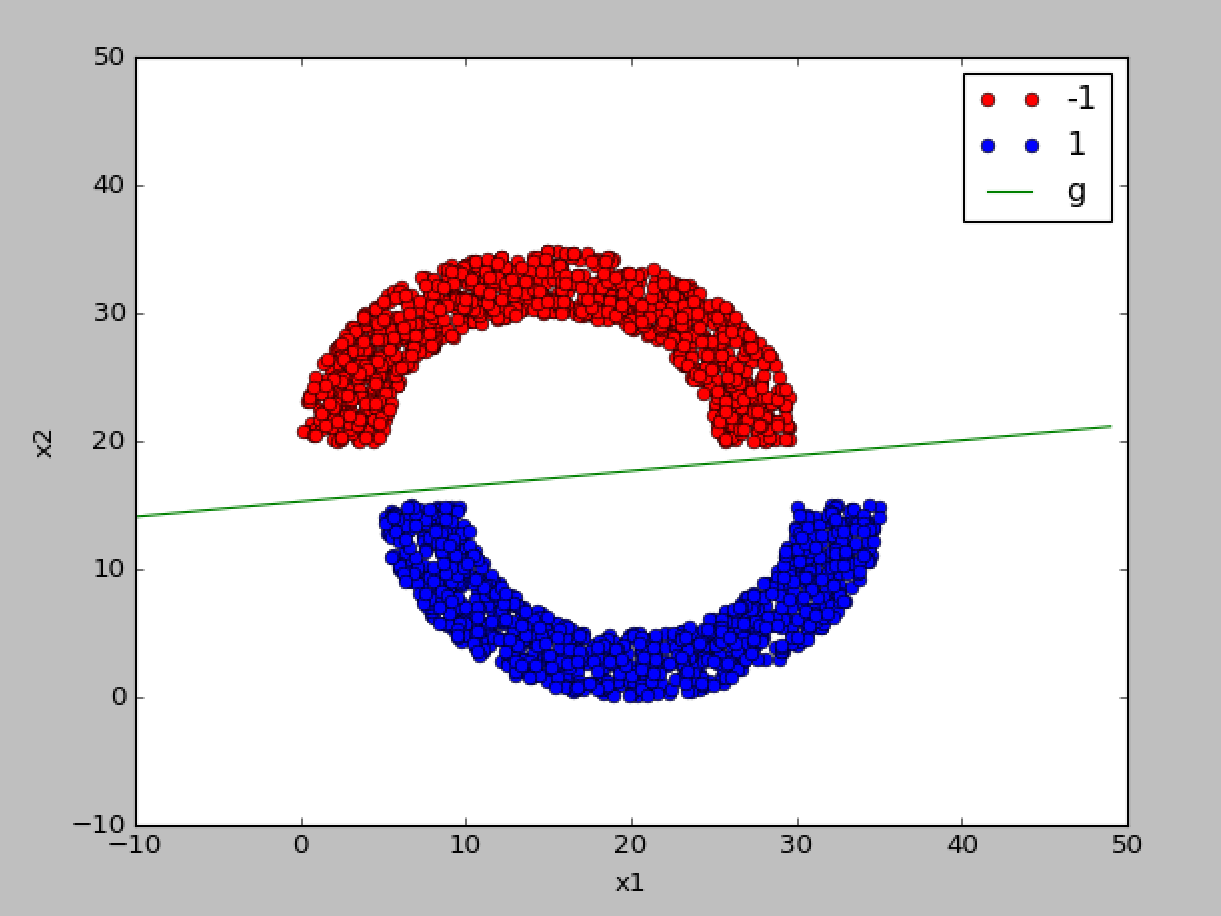
\includegraphics[scale=.5]{3-1a.png}
	\\ The above image is the display after running the PLA algorithm on 2000 generated points. It terminated after 1137 iterations, with output function $x_2 = .1195x_1 + 15.274$
	\item 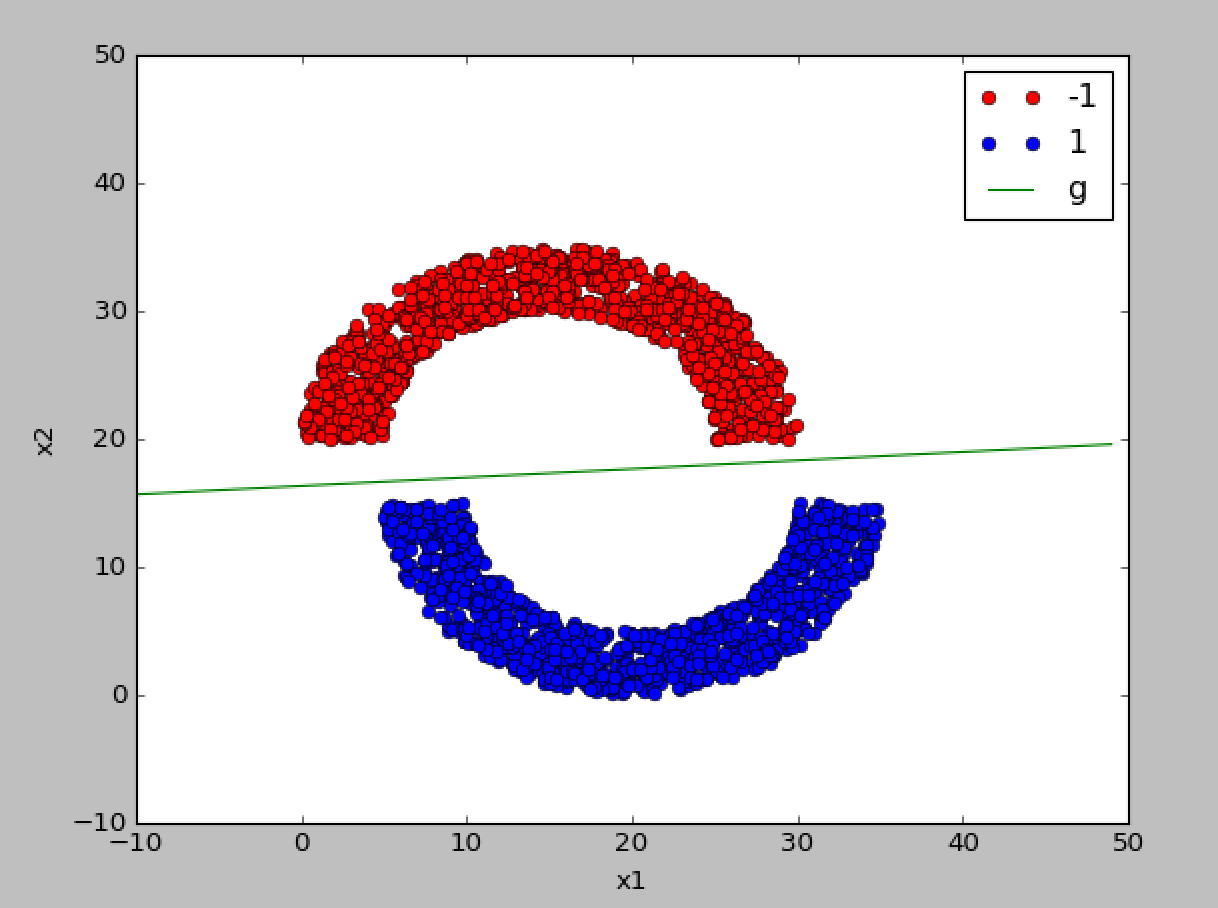
\includegraphics[scale=.5]{3-1b.png}
	\\ The above image is the display after running the linear regression algorithm described in the chapter on 2000 generated points. It runs extremely quickly with very high accuracy. Sometimes when running the PLA it would be very volatile in its termination time (see 3.2 below), but this algorithm was very consistently quick. Its output was $x_2 = .0664x_1 + 16.335$
\end{enumerate}
\section*{Problem 3.2}
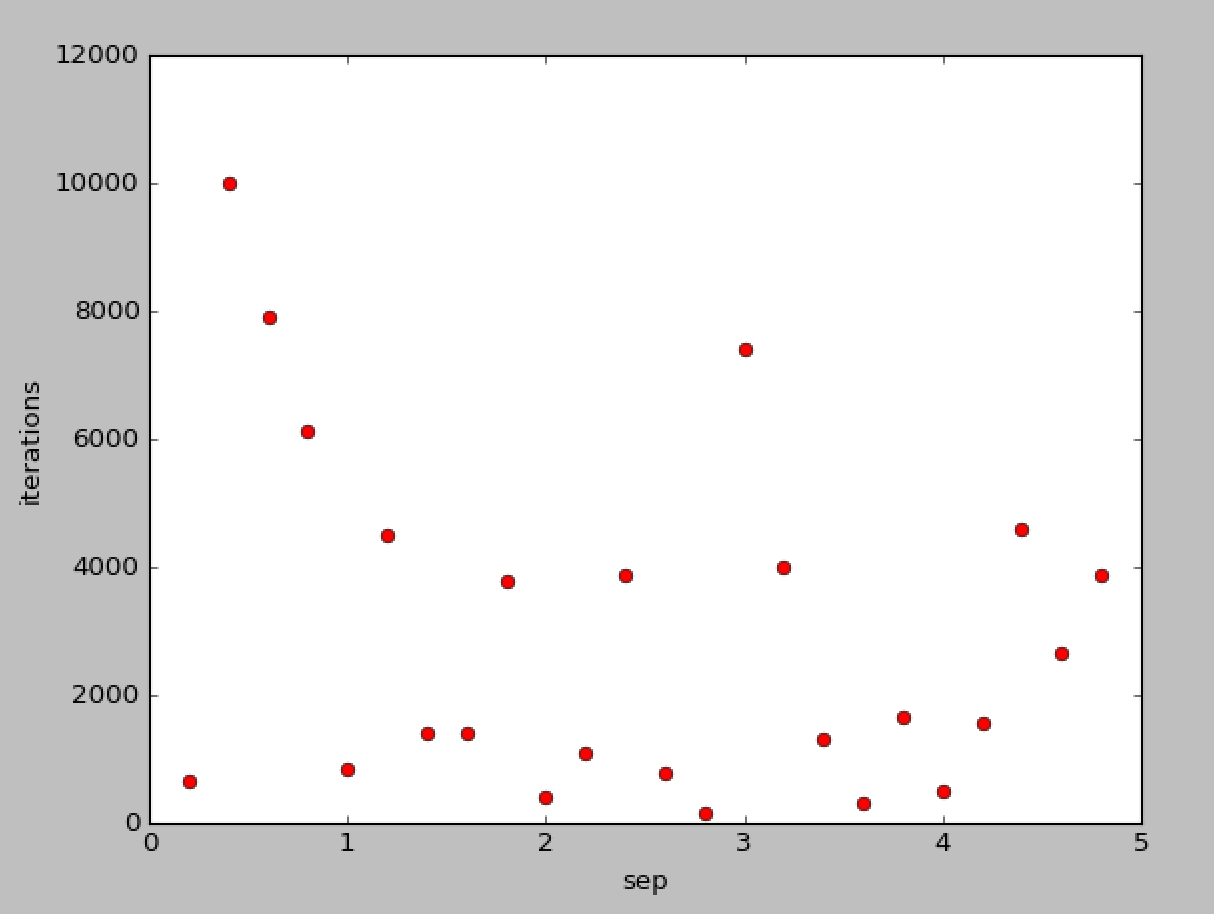
\includegraphics[scale=.5]{3-2.png}
\\ The above image is the output after graphing sep (the vertical separation between the semicircles) versus the number of iterations PLA took to terminate. There isn't really any super visible trend, except for a mild inverse relationship between sep and iterations.
\\ \\ Both of these things are expected. PLA is a somewhat volatile algorithm, because its performance can really hinge on which points it ends up picking to re-evaluate its weights on. However, the weak inverse relationship intuitively makes sense because as the sep gets bigger, there are more possible hypotheses that can separate the data.
\\ \\ Meanwhile, the bound we proved back in problem 1.3e, where $t < \frac{R^2||w^*||^2}{\rho}$, doesn't really change that much. The norm of the optimal weight vector doesn't change very much, but R and $\rho$ both increase as sep increases. This is because as sep increases, the distance points get from the termination line increases. Both increase with a squared factor, so the bound will not shift too much.
\section*{Problem 3.8}
We can simplify the expression given in the problem as follows:
\begin{gather*}
	E_{out}(h) = E[(h(x) - y)^2]
	\\ = h^2(x) - 2h(x)E[y|x] + E[y^2|x]
	\\ \frac{dE_{out}}{dh(x)} = 2h(x) - 2E[y|x] = 0
	\\ \implies \boldsymbol{h(x) = E[y|x]}
\end{gather*}
We can also show that $E[\epsilon(x)] = 0$ in the following way:
\begin{gather*}
	y = h^*(x) + \epsilon(x)
	\\ E[y] = E[h^*(x) + \epsilon(x)]
	\\ E[y] = E[h^*(x)] + E[\epsilon(x)]
	\\ E[y] = h^*(x) \implies h^*(x) = h^*(x) + E[\epsilon(x)]
	\\ \implies \boldsymbol{E[\epsilon(x)] = 0}
\end{gather*}
\section*{Extra Problem}
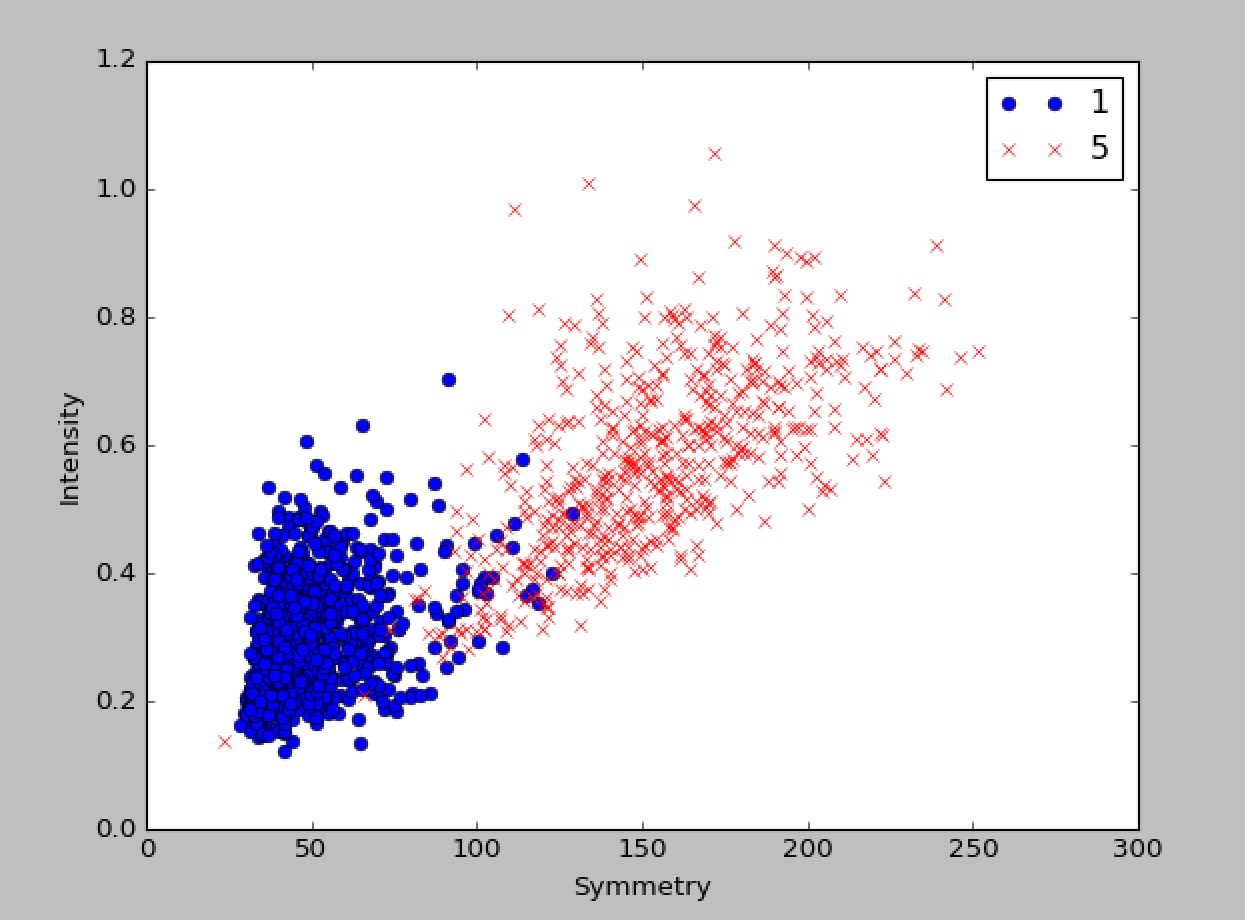
\includegraphics[scale=.75]{extra.png}
\\ 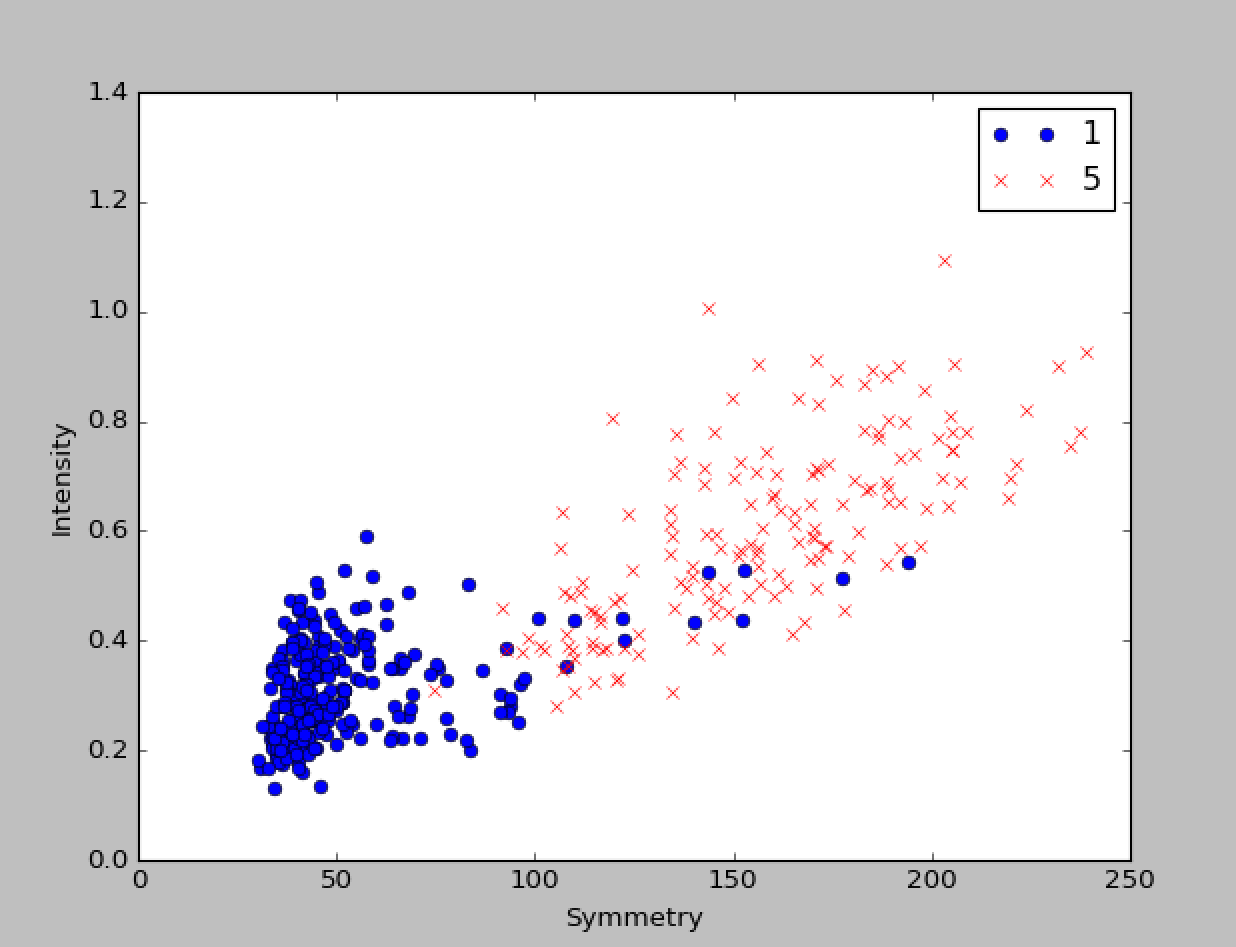
\includegraphics[scale=.75]{extra2.png}
\\ The above two graphs depict symmetry vs. intensity for the training and test data sets respectively.
\\ \\ Symmetry was defined as the picture's symmetry about both the x-axis and the y-axis. Mathematically speaking, symmetry was calculated as (with $P[n]$ representing the nth index of the input grayscale image, i being column and j being row number of specific pixels):
\begin{gather*}
\sum_{0 \le i \le 7, 0 \le j \le 16}|P[16j + i] - P[16(j + 1) - (i + 1)]| + 
\\ \sum_{0 \le i \le 16, 0 \le j \le 7}^{15}|P[16j + i] - P[(15 - j)*16 - i]
\end{gather*}
Essentially, images were penalized for having pixels that differed much in value from the corresponding pixel on the other side of either the y or x axis.
\\ \\ Average intensity was done by taking the difference between each pixel and pure white (-1), summing and averaging everything. Mathematically, this turned out to be:
\begin{gather*}
\frac{1}{256}\sum_{0 \le i < 256}P[i] + 1
\end{gather*}
This turned out to have pretty decent performance. Unfortunately, there are a few clear outliers even if the main chunk of all the points are well separated.
\end{document}